\section{代數數、超越數，與 $\e$ 這個數}\label{sec:numbers}

\subsection{代數數與超越數}

\begin{prereq}{代數數（algebraic number）與超越數（transcendental number）}
一個複數 $\alpha$ 叫做\textbf{代數數}，如果存在一個\emph{不是零多項式}的整數係數多項式
$f(x)=a_0+a_1x+\cdots+a_nx^n$（$a_i\in\Z$），使得 $f(\alpha)=0$。
不是代數數的複數叫做\textbf{超越數}。
\end{prereq}

\begin{exmp}
\begin{itemize}
  \item 每個有理數都是代數數：$\tfrac{3}{7}$ 是 $7x-3=0$ 的根。
  \item $\sqrt2$ 是代數數：它是 $x^2-2=0$ 的根。$\sqrt[3]{5}$ 是 $x^3-5=0$ 的根。
  \item 虛數單位 $i$ 是代數數：$x^2+1=0$。黃金比例 $\tfrac{1+\sqrt5}{2}$ 是 $x^2-x-1=0$ 的根。
  \item $\sqrt2+\sqrt3$ 也是代數數。令 $x=\sqrt2+\sqrt3$，則 $x^2=5+2\sqrt6$，
        $(x^2-5)^2=24$，所以 $x$ 是 $x^4-10x^2+1=0$ 的根。
\end{itemize}
\end{exmp}

所以「$\e$ 是超越數」的意思，就是導讀開頭寫的那句話：不論整數 $a_0,\ldots,a_n$（不全為零）怎麼取，都有 $a_0+a_1\e+\cdots+a_n\e^n\neq0$。
論文的每一個證明都從「假設它等於 $0$」出發，推出矛盾，這就是高中學過的\textbf{反證法}。

\begin{figure}[htbp]
\centering
\begin{tikzpicture}[font=\small]
  \draw[fill=gray!8, rounded corners=8pt] (-5.6,-2.3) rectangle (5.6,2.3);
  \node[anchor=north west] at (-5.5,2.25) {複數 $\C$};
  \draw[fill=orange!15, rounded corners=8pt] (-5.2,-1.75) rectangle (1.9,1.75);
  \node[anchor=north west] at (-5.1,1.7) {代數數};
  \draw[fill=blue!10, rounded corners=6pt] (-4.8,-1.2) rectangle (-0.6,1.2);
  \node[anchor=north west] at (-4.7,1.15) {有理數 $\Q$};
  \draw[fill=blue!22, rounded corners=5pt] (-4.4,-0.7) rectangle (-1.4,0.7);
  \node at (-2.9,0.15) {整數 $\Z$};
  \node at (-2.9,-0.35) {\footnotesize $0,\pm1,\pm2,\ldots$};
  \node at (0.6,0.6) {$\sqrt2$};
  \node at (1.2,-0.2) {$i$};
  \node at (0.4,-0.9) {$\sqrt2+\sqrt3$};
  \node[text=red!70!black] at (3.8,1.1) {$\e$};
  \node[text=red!70!black] at (3.2,0.1) {$\pi$};
  \node[text=red!70!black] at (4.3,-0.6) {$\e^{\pi}$};
  \node[text=red!70!black] at (3.4,-1.4) {$2^{\sqrt2}$};
  \node[anchor=south east, text=red!70!black] at (5.5,-2.25) {超越數（代數數以外的全部）};
\end{tikzpicture}
\caption{數的分類。代數數包含所有有理數和所有「根號式」。超越數是其餘的複數；
圖中列出的四個都已被證明是超越數（$\e^\pi$ 與 $2^{\sqrt2}$ 由 Gelfond--Schneider 定理，1934）。}
\label{fig:classes}
\end{figure}

\paragraph{一點歷史。}
1844 年 Liouville 造出第一個超越數（$\sum_{k\ge1}10^{-k!}=0.110001000\ldots$）。
1873 年 Hermite 證明 $\e$ 是超越數，這是第一個「自然出現的」超越數。
1882 年 Lindemann 用同樣的方法證明 $\pi$ 是超越數，順便解決了兩千年來的「化圓為方」問題。
1893 年希爾伯特把兩個證明精簡成幾頁，論文第一節複述的就是這個版本。
另外，1874 年 Cantor 證明超越數「多到數不完」，但他的證明不會告訴你任何一個具體的超越數是誰；
這和本文第 \ref{sec:countable} 節的「可數／不可數」有關。

\subsection{$\e$ 是什麼？指數級數}

高中課本把 $\e$ 當成「自然對數的底」，大約是 $2.71828$。本篇論文則把 $\e$ 和指數函數
看成一個\emph{無窮級數}，這是接下來一切的起點。

\begin{prereq}{$\e$ 與 $\e^x$ 的級數定義}
\[
  \e:=\sum_{n\ge0}\frac{1}{n!}=1+1+\frac12+\frac16+\frac1{24}+\cdots,\qquad
  \e^{x}:=\sum_{n\ge0}\frac{x^n}{n!}=1+x+\frac{x^2}{2}+\frac{x^3}{6}+\cdots\quad(x\in\R)\,.
\]
這兩個無窮和都收斂（會逼近一個固定的數）。原因：當 $n$ 夠大時，相鄰兩項的比值
$\dfrac{x^{n+1}/(n+1)!}{x^n/n!}=\dfrac{x}{n+1}$ 的絕對值小於 $\tfrac12$，
所以從某一項開始，後面的項比一個公比 $\tfrac12$ 的等比級數還小，而等比級數是收斂的。
\end{prereq}

\begin{figure}[htbp]
\centering
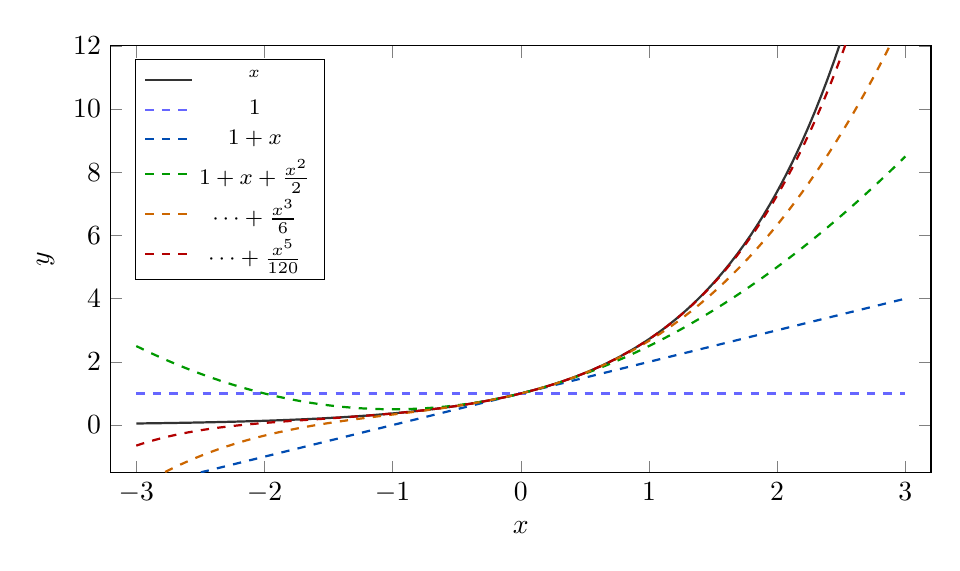
\begin{tikzpicture}
\begin{axis}[width=12cm, height=7cm, xmin=-3.2, xmax=3.2, ymin=-1.5, ymax=12,
  xlabel={$x$}, ylabel={$y$}, legend pos=north west, legend style={font=\footnotesize},
  samples=120, domain=-3:3, no markers, every axis plot/.append style={thick}]
  \addplot[black!80] {exp(x)};
  \addplot[blue!60, dashed] {1};
  \addplot[blue!70!green, dashed] {1+x};
  \addplot[green!60!black, dashed] {1+x+x^2/2};
  \addplot[orange!80!black, dashed] {1+x+x^2/2+x^3/6};
  \addplot[red!70!black, dashed] {1+x+x^2/2+x^3/6+x^4/24+x^5/120};
  \legend{$\e^x$, $1$, $1+x$, $1+x+\frac{x^2}{2}$, $\cdots+\frac{x^3}{6}$, $\cdots+\frac{x^5}{120}$}
\end{axis}
\end{tikzpicture}
\caption{$\e^x$ 的級數部分和。每多加一項，曲線在更大的範圍內貼近 $\e^x$。
在 $x=1$ 處，前 $13$ 項的和已經是 $2.7182818283$，和 $\e$ 的前十位小數相同。}
\label{fig:expseries}
\end{figure}

\begin{prereq}{從級數推出 $\e^{a+b}=\e^a\e^b$}
論文多次使用「指數律」$\e^{a+b}=\e^{a}\e^{b}$（第一節算 $B_r$ 時，以及第三節的命題 3.6）。
它可以直接從級數和\textbf{二項式定理}推出：
\begin{align*}
  \e^{a+b}=\sum_{n\ge0}\frac{(a+b)^n}{n!}
  &=\sum_{n\ge0}\sum_{k=0}^{n}\frac{1}{n!}\binom{n}{k}a^kb^{n-k}
  =\sum_{n\ge0}\sum_{k=0}^{n}\frac{a^k}{k!}\cdot\frac{b^{n-k}}{(n-k)!}\\
  &=\Big(\sum_{k\ge0}\frac{a^k}{k!}\Big)\Big(\sum_{l\ge0}\frac{b^l}{l!}\Big)=\e^a\e^b\,.
\end{align*}

中間用了 $\frac{1}{n!}\binom nk=\frac{1}{k!\,(n-k)!}$，最後一步是把「所有 $(k,l)$ 的乘積」
按 $k+l=n$ 分組。這種「重新分組」在第 \ref{sec:fps} 節會再出現，它正是兩個冪級數相乘的規則。
\end{prereq}

另一個會用到的性質：$\e^x$ 的導數還是 $\e^x$。逐項微分
$\big(\tfrac{x^n}{n!}\big)'=\tfrac{x^{n-1}}{(n-1)!}$，所以整個級數微分後只是「每一項往前移一格」，
形狀不變。於是 $(\e^{-x})'=-\e^{-x}$，這在第 \ref{sec:calc} 節的分部積分裡會用到。

\subsection{階乘打敗指數：$c^r/r!\to0$}\label{sec:factorial}

三個證明最後都靠同一個事實收尾：\emph{階乘的成長速度終究會超過任何固定底數的指數。}

\begin{prereq}{$c^r/r!\to0$}
固定任何一個實數 $c\ge1$。當 $r\to\infty$ 時，$\dfrac{c^r}{r!}\to0$。

\textbf{理由。}取一個整數 $R>2c$。當 $r\ge R$ 時，
\[
  \frac{c^{r}}{r!}=\frac{c^{R}}{R!}\cdot\frac{c}{R+1}\cdot\frac{c}{R+2}\cdots\frac{c}{r}
  \le\frac{c^{R}}{R!}\cdot\Big(\frac12\Big)^{r-R}\,,
\]
因為每個額外的因子 $\frac{c}{R+j}$ 都小於 $\frac12$。右邊是一個固定常數乘上 $(\tfrac12)^{r-R}$，
當然趨近於 $0$。同理，對任何固定的 $A\ge1$，當 $k$ 夠大時 $k!>A^k$；
論文第二節需要的形式是：存在 $k_0$，使得 $k\ge k_0$ 時 $k!>c\,A^{2tk}C^{k}=c\,(A^{2t}C)^k$。
\end{prereq}

\begin{figure}[htbp]
\centering
\begin{tikzpicture}
\begin{axis}[width=12cm, height=6.8cm, xmin=0, xmax=41, ymin=0, ymax=50,
  xlabel={$r$}, ylabel={$\log_{10}$（位數）}, legend pos=north west,
  legend style={font=\footnotesize}, no markers, every axis plot/.append style={thick}]
  \addplot[blue!70!black, domain=0:40, samples=2] {x};
  \addplot[red!70!black, mark=*, mark size=1pt] coordinates {
    (0,0.000) (1,0.000) (2,0.301) (3,0.778) (4,1.380) (5,2.079) (6,2.857) (7,3.702)
    (8,4.606) (9,5.560) (10,6.560) (11,7.601) (12,8.680) (13,9.794) (14,10.940)
    (15,12.116) (16,13.321) (17,14.551) (18,15.806) (19,17.085) (20,18.386)
    (21,19.708) (22,21.051) (23,22.412) (24,23.793) (25,25.191) (26,26.606)
    (27,28.037) (28,29.484) (29,30.947) (30,32.424) (31,33.915) (32,35.420)
    (33,36.939) (34,38.470) (35,40.014) (36,41.571) (37,43.139) (38,44.719)
    (39,46.310) (40,47.912)};
  \legend{$10^{r}$, $r!$}
  \draw[dashed, gray] (axis cs:25,0) -- (axis cs:25,25.2);
  \node[font=\footnotesize, anchor=west] at (axis cs:25.5,8) {$r=25$ 之後 $r!$ 反超};
\end{axis}
\end{tikzpicture}
\caption{以 $c=10$ 為例，比較 $10^{r}$ 與 $r!$ 的位數。$10^r$ 每多一步只多一位，
$r!$ 每多一步多 $\log_{10}r$ 位，越走越快。}
\label{fig:factorial}
\end{figure}

\subsection{暖身：核心招數，用它證明 $\e$ 是無理數}\label{sec:irrational}

三個證明的靈魂都是下面這個招數。我們先用它做一件高中生做得到的事。

\begin{keyidea}[核心招數：非零整數的絕對值至少是 $1$]
如果你能證明某個數 $N$ 同時滿足
\begin{enumerate}
  \item $N$ 是整數，而且 $N\neq0$；
  \item $|N|<1$，
\end{enumerate}
那就矛盾了。希爾伯特證明裡的 $N$ 是 $B_r/r!$（或等價地 $-A_r/r!$），
第二節的 $N$ 是 $v_n(k)/k!$。
\end{keyidea}

\begin{thm}[Fourier, 1815]
$\e$ 是無理數。
\end{thm}
\begin{pf}
假設 $\e=\dfrac{p}{q}$，$p,q\in\N$。把 $\e=\sum_{n\ge0}\frac1{n!}$ 乘上 $q!$：
\[
  q!\,\e=\underbrace{q!\Big(1+1+\frac1{2!}+\cdots+\frac1{q!}\Big)}_{\text{整數，記作 }M}
        +\underbrace{q!\Big(\frac{1}{(q+1)!}+\frac{1}{(q+2)!}+\cdots\Big)}_{\text{記作 }T}\,.
\]
左邊 $q!\,\e=(q-1)!\,p$ 是整數，$M$ 是整數，所以 $T=q!\,\e-M$ 也是整數。但是
\[
  0<T=\frac{1}{q+1}+\frac{1}{(q+1)(q+2)}+\cdots<\frac1{q+1}+\frac1{(q+1)^2}+\cdots=\frac1q\le1\,.
\]
$T$ 是嚴格介於 $0$ 與 $1$ 之間的整數，矛盾。
\end{pf}

請注意這個證明的骨架：「乘上一個大階乘，把級數拆成\emph{整數部分}與\emph{尾巴}，
尾巴非零但比 $1$ 小」。希爾伯特的證明是它的加強版：把「乘上 $q!$」換成「乘上一個
精心設計的積分」，讓拆出來的整數部分是 $r!$ 的倍數，而尾巴只有 $c^r$ 那麼大。
第二節的證明也是同一骨架，只是把「尾巴很小」這件事藏在 $v_n=O(A^n)$ 裡。
